% ---------------------------------------------------------------------------
% Author guideline and sample document for EG publication using LaTeX2e input
% D.Fellner, v1.13, Nov 13, 2007

\documentclass{egpubl}

% --- for  Annual CONFERENCE
\VisualComputing % VisualComputing (added by U. Schwanecke, 2021)
%\ThreeDAnimation % 3DAnimation (added by U. Schwanecke, 2020)
%\Seminar % Specialist Seminar (added by U. Schwanecke, 2019)
%\ConferenceSubmission % uncomment for Conference submission
%\ConferencePaper      % uncomment for (final) Conference Paper
%\STAR                 % uncomment for STAR contribution
% \Tutorial             % uncomment for Tutorial contribution
% \ShortPresentation    % uncomment for (final) Short Conference Presentation
%
% --- for  CGF Journal
% \JournalSubmission    % uncomment for submission to Computer Graphics Forum
% \JournalPaper         % uncomment for final version of Journal Paper
%
% --- for  CGF Journal: special issue
% \SpecialIssueSubmission    % uncomment for submission to Computer Graphics Forum, special issue
% \SpecialIssuePaper         % uncomment for final version of Journal Paper, special issue
%
% --- for  EG Workshop Proceedings
% \WsSubmission    % uncomment for submission to EG Workshop
% \WsPaper         % uncomment for final version of EG Workshop contribution
%
%\electronicVersion % can be used both for the printed and electronic version

% !! *please* don't change anything above
% !! unless you REALLY know what you are doing
% ------------------------------------------------------------------------

\PrintedOrElectronic

\usepackage[pdftex]{graphicx} 
\usepackage{t1enc, dfadobe}
%\usepackage[T1]{fontenc}
\usepackage{egweblnk}
\usepackage{cite}

% For backwards compatibility to old LaTeX type font selection.
% Uncomment if your document adheres to LaTeX2e recommendations.
% \let\rm=\rmfamily    \let\sf=\sffamily    \let\tt=\ttfamily
% \let\it=\itshape     \let\sl=\slshape     \let\sc=\scshape
% \let\bf=\bfseries

% end of prologue

\usepackage{blindtext}
\usepackage{caption}
\usepackage{subfigure}
\usepackage{dblfloatfix}
\usepackage{adjustbox}
\usepackage{mathtools}
\usepackage{todonotes}


% ---------------------------------------------------------------------
\captionsetup{labelfont=bf,textfont=it}
\title[Burst Images]%
      {Burst Images}

\author[Sascha Scheid]
    {\parbox{\textwidth}
        {\centering 
			Sascha Scheid
        }
        \\
    {\parbox{\textwidth}
        {\centering RheinMain University of Applied Sciences, Wiesbaden, Germany\\
       }
    }
}
% ------------------------------------------------------------------------

% if the Editors-in-Chief have given you the data, you may uncomment
% the following five lines and insert it here
%
% \volume{36}   % the volume in which the issue will be published;
% \issue{1}     % the issue number of the publication
% \pStartPage{1}      % set starting page


%-------------------------------------------------------------------------
\begin{document}

%-------------------------------------------------------------------------
% uncomment for using teaser (comment if you don't want a teaser)
\teaser{
    \hspace{\fill}
    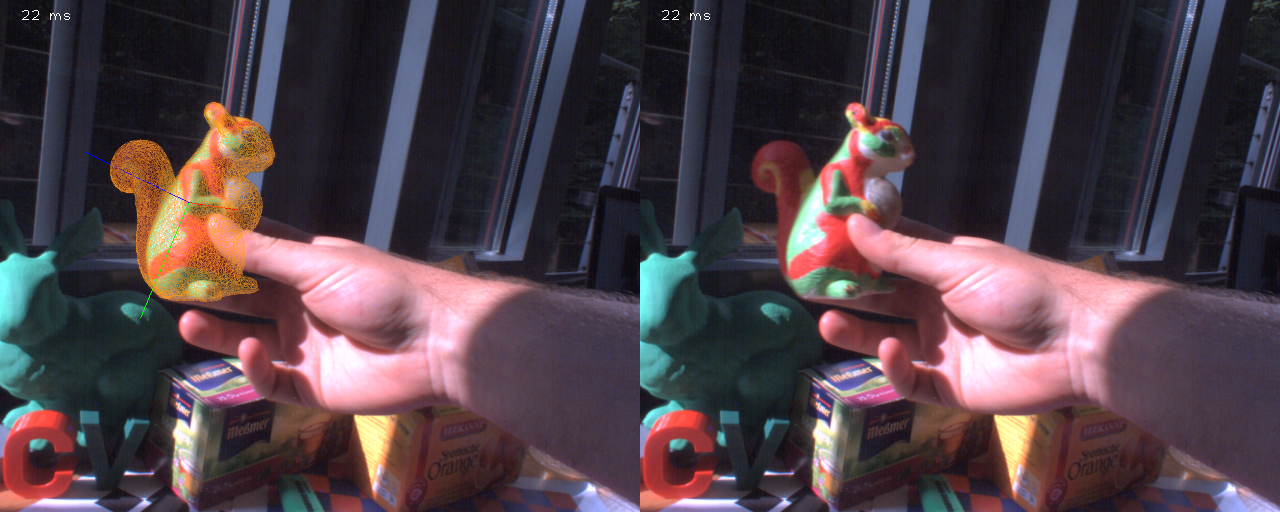
\includegraphics[width=0.9\linewidth]{images/ModelbasedTrackingExample.png}
    \hspace{\fill}
    \centering
    \caption{Best teaser image you can provide \ldots}
    \label{fig:teaser}
}


%-------------------------------------------------------------------------
\maketitle


%-------------------------------------------------------------------------
\begin{abstract}
Some informative abstract \ldots
\blindtext
\end{abstract}  


%-------------------------------------------------------------------------
\section{Introduction}
\label{sec:introduction}

Burst photography is a technique in which a series of photographs is taken quickly in succession.
This can be useful in a variety of situations, such as capturing action or movement, 
or to create a sense of motion. In digital photography, burst images are stored as a 
sequence of image files, typically in a format such as JPEG or RAW.

High Dynamic Range (HDR) is a technique used to improve the dynamic range of an image, 
which is the range of luminance or brightness levels that can be captured in a photograph. 
The dynamic range of a scene can often be greater than what a camera is able to capture 
in a single image, resulting in lost detail in the highlights or shadows. 
HDR techniques can be used to extend the range of luminance in an image, 
resulting in more detail and a more realistic representation of the scene.

One way that burst photography and HDR techniques can be used together
is to capture a series of photographs with different exposures in a burst, and then combine 
the exposures into a single HDR image using software. This can be particularly useful in 
low-light situations, where the camera may struggle to capture a wide range of luminance 
levels in a single exposure. By capturing multiple exposures and combining them into an 
HDR image, it is possible to extend the dynamic range and capture more detail in both the 
highlights and shadows.

\cite{Hasinoff2016Burst}



%-------------------------------------------------------------------------
\section{Related Work}
\label{sec:related_work}
Maybe a separate section about related work \ldots 
\blindtext


%-------------------------------------------------------------------------
\section{Approach}
\label{sec:approach}
\blindtext


%-------------------------------------------------------------------------
\section{Experiments}
\label{sec:Experiments}
\blindtext


%-------------------------------------------------------------------------
\section{Conclusions}
\label{sec:conclusion}
Some famous last words \ldots
\blindtext


%-------------------------------------------------------------------------
\section{Acknowledgements}
\label{sec:acknowledgements}
Maybe you like to acknowledge \ldots 


%-------------------------------------------------------------------------
%\bibliographystyle{eg-alpha}
\bibliographystyle{eg-alpha-doi}
\bibliography{paper-bib}

\end{document}